% vim: set tw=78 sts=2 sw=2 ts=8 aw et ai:

Wireless sensor network consist of numerous autonomous sensors that are
capable of monitoring the environment in which they are placed with various
sensors. Such network would be usefull for such things as polution monitoring
in a city or poisonous gases or might be able to sense vibrations to predict
an earthquake. 

An wireless sensor network will contain many nodes, anywhere from a couple
hundred sensors to several thounds nodes. Each one of this nodes has one or
more sensors for getting data from the environment, the number being limited
by size and power consumption. They also have a microcontroller to process the
data from the sensor and a tranceiver to be able send to some sink-node the
data it collected. They are usually powered by some sort of battery although
solar cells and capacitors have also been used.

Each sensor collects data from it's location and sends it to the base station,
from where data from the whole network can be collected. It is very power
consuming to send data over long distances as the tranciever will need to
amplify the power more so this should be avoided if possible by sending to
closer nodes. This is from where the need of routing protocols for these
networks come. Instead of sending data directly to the base station, the nodes
group in an hierarchical way so that each node will send data to a cluster
head that is very close which then sends it to the base station or to a higher
order cluster head.

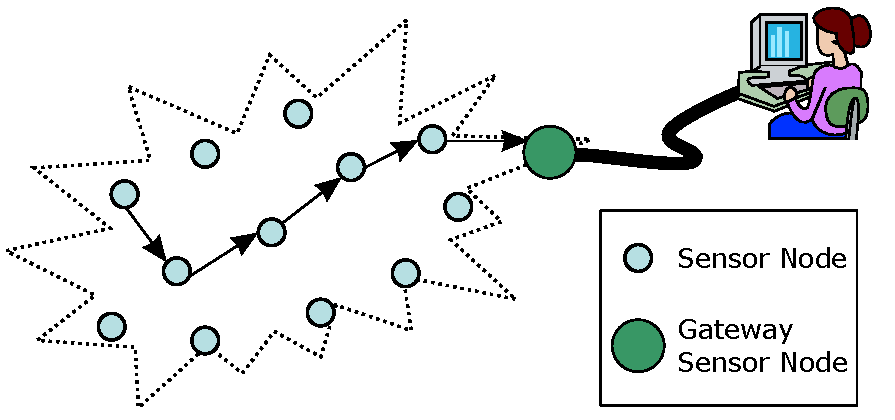
\includegraphics{img/WSN.pdf}
\\
In this paper we will present some of the existing Wireless Network
Simulators emphasizing what we believe to be their strenghts and weaknesses. 
In section NS-2 we discuss about NS-2 simulator, in section J-sim we present
J-sim and then we take a look at TOSSIM simulator. Based on these observations
we introduce in section \codename  the WSN simulator we will implement which
encompasses most of these simulators' strenghts and adds some new features
for wireless network simulators.
